% It is an example file showing how to use the 'sigkddExp.cls' 
% LaTeX2e document class file for submissions to sigkdd explorations.
% It is an example which *does* use the .bib file (from which the .bbl file
% is produced).
% REMEMBER HOWEVER: After having produced the .bbl file,
% and prior to final submission,
% you need to 'insert'  your .bbl file into your source .tex file so as to provide
% ONE 'self-contained' source file.
%
% Questions regarding SIGS should be sent to
% Adrienne Griscti ---> griscti@acm.org
%
% Questions/suggestions regarding the guidelines, .tex and .cls files, etc. to
% Gerald Murray ---> murray@acm.org
%

\documentclass{article}
\usepackage{cite}
\usepackage{amssymb}
\usepackage{amsmath}
\usepackage{amsfonts}
\usepackage{algorithm}
\usepackage{algpseudocode}

\usepackage{tikz}
\usetikzlibrary{shapes.geometric, arrows}

\renewcommand{\algorithmicrequire}{\textbf{Input:}}
\renewcommand{\algorithmicensure}{\textbf{Output:}}

\tikzstyle{startstop} = [rectangle, rounded corners, minimum width=3cm, minimum height=1cm,text centered, draw=black]
\tikzstyle{io} = [trapezium, trapezium left angle=70, trapezium right angle=110, minimum width=3cm, minimum height=1cm, text centered, draw=black]
\tikzstyle{process} = [rectangle, minimum width=3cm, minimum height=1cm, text centered, text width=3cm, draw=black]
\tikzstyle{decision} = [diamond, minimum width=3cm, minimum height=1cm, text centered, draw=black]
\tikzstyle{arrow} = [thick,->,>=stealth]



\begin{document}

%
% --- Author Metadata here ---
% -- Can be completely blank or contain 'commented' information like this...
%\conferenceinfo{WOODSTOCK}{'97 El Paso, Texas USA} % If you happen to know the conference location etc.
%\CopyrightYear{2001} % Allows a non-default  copyright year  to be 'entered' - IF NEED BE.
%\crdata{0-12345-67-8/90/01}  % Allows non-default copyright data to be 'entered' - IF NEED BE.
% --- End of author Metadata ---

\title{Online Distributed Bootstrap for Big Data}
\author{William High}
\date{\today}
\maketitle

\begin{abstract}

This document outlines an Online Bag of Little Bootstraps (OBLB) idea. The Bag
of Little Bootstraps is useful for static, distributed data, but requires you
to know the total data set size and the size of each split on the distributed
nodes. The OBLB variant presented here does not require the total data set
size to be known, nor the size of splits, and in fact the data can be
unbounded.

\end{abstract}

\section{Bootstrap}

The original bootstrap is by \cite{bib:efron}. This is the basic,
nonparametric bootstrap involving resampling $n$ data points with replacement
$n$ times in $r$ total iterations, where $r \gtrsim 200$. An analysis pipeline
is executed at each bootstrap iteration, and a histogram of a resulting
statistic is built up in the process. The histogram is an estimator of the
sample distribution of that statistic. As a result, the mean of the bootstrap
distribution is an estimate of the sample mean; the standard deviation is an
estimate of the standard error on the mean; confidence intervals are computed
on the histograms directly; and covariance on multivariate statistics can be
computed on the joint bootstrap distribution directly.

\section{Online Bootstrap}

The online bootstrap (OB) is sketched by \cite{bib:onlineboot} and is
incorporated into Vowpal Wabbit. Those authors noted that the number of times
a single data point is resampled in one iteration of the traditional bootstrap
is distributed as $Poisson(\lambda = 1)$ for reasonable $r$. This suggests
using an importance weight $W = w^{\prime}w$ for each data point in a stream,
where $w^{\prime}$ is the input importance weight of the data point and $w
\sim Poisson(\lambda = 1)$ is a weight that emulates bootstrap resampling.

\section{Bag of Little Bootstraps}

The Bag of Little Bootstraps is by \cite{bib:blb}. These authors had in mind
big data that is split across nodes, such as on the Hadoop Filesystem. The BLB
procedure is to run the bootstrap on each node that can locally access,
compute a statistic (e.g.\ the mean, confidence interval) on each bootstrap
distribution separately, then collect the statistic from each node and average
to produce a global statistic.

As stated, the method requires that you know the size of each data split and
the total size of the data set, and that you can compute and store a reservoir
of resample indexes in memory. It also makes the interesting choice of
aggregating up the bootstrap distribution to a summary statistic on each node,
and then average each summary statistic, which speeds up the algorithm but
doesn't allow for the mining of additional bootstrap distribution summary
statistics after the fact.

\section{Online Bag of Little Bootstraps}

Given that $r$ is typically chosen to be of order $10^2$ to $10^4$ or so, it's
reasonable to aggregate and persist $r$ bootstrap buckets on a node or set of
nodes using an online bootstrap bucket update rule.

The inner bootstraps require an online update rule that respects importance
weights. The outer bootstrap aggregator requires a different

Algorithm \ref{onlineblb} outlines the OBLB idea.

\begin{algorithm}
\caption{Online distributed bootstrap}
\label{onlineblb}
\begin{algorithmic}[1]
\Require \\
Unbounded set of data-weight tuples $\{(X_1,w^{\prime}_1), (X_2,w^{\prime}_2), ...\}$\\
Number of bootstrap buckets $r$\\
Data split nodes $\{1,2, ..., s\}$, plus a master bootstrap node\\
Online estimator update rule OnlineUpdate
\Ensure \\
Estimator value in each bootstrap bucket, $\hat\theta_{k}\;\forall \; k\in \{1, 2, ...., r\}$
\Procedure{Online Distributed Bootstrap}{}
\State // Initialize the estimators and weights.
\For{each bootstrap instance $k \gets 1$ to $r$}
\State $w_{k} \gets 0$
\State $\hat\theta_{k} \gets 0$
\State // $s$ nodes maintain independent bootstrap buckets $\hat\theta_{jk}$ with associated weights $w_{jk}$.
\For{each node $j \gets 1$ to $s$}
\State $w_{jk} \gets 0$
\State $\hat\theta_{jk} \gets 0$
\EndFor
\EndFor
\State // Stream through the data.
\For{each $i \gets 1$ to $\infty$}
\State Randomly assign tuple $(X_i,w^{\prime}_i)$ to node $j \in \{1, 2, ..., s\}$
\State // $s$ nodes maintain $r$ independent bootstraps.
\State // Update the bootstrap buckets on node $j$:
\For{each $k \gets 1$ to $r$}
\State $W \gets w^{\prime}_i \times Poisson(\lambda = 1)$
\State $(\hat\theta_{jk}, w_{jk}) \gets \mathrm{OnlineUpdate}(\hat\theta_{jk}, w_{jk}, X_i, W)$
\EndFor
\State // Another node maintains $r$ master bootstrap aggregates.
\State // Update the bootstrap buckets on the master bootstrap node:
\For{each $k \gets 1$ to $r$}
\State $(\hat\theta_{k}, w_{k}) \gets \mathrm{OnlineMasterUpdate}(\hat\theta_{k}, w_{k},\hat\theta_{jk}, w_{jk})$
\EndFor
\EndFor
\EndProcedure
\end{algorithmic}
\end{algorithm}

Algorithm \ref{onlineupdate} is an example online update rule. Another example
from a machine learning application is the Vowpal Wabbit online trainer.

\begin{algorithm}
\caption{OnlineUpdate example: streaming mean}
\label{onlineupdate}
\begin{algorithmic}[1]
\Require \\
Current mean $\theta_0$ \\
Aggregate weight of current mean $w_0$ \\
New data $X$ \\
Weight of new data $w$
\Ensure \\
Updated mean $\theta_1$ \\
Aggregate weight of updated mean $w_1$
\Procedure{OnlineUpdate}{}
\State $\theta_1 \gets (w_0\theta_0 + WX)/(w_0 + W)$
\State $w_1 \gets w_0 + W$ 
\State \Return $(\theta_1, w_1)$
\EndProcedure
\end{algorithmic}
\end{algorithm}

A flowchart is shown in Figure \ref{oblbflowchart}.

\begin{figure}[tbp]
\centering
\label{oblbflowchart}
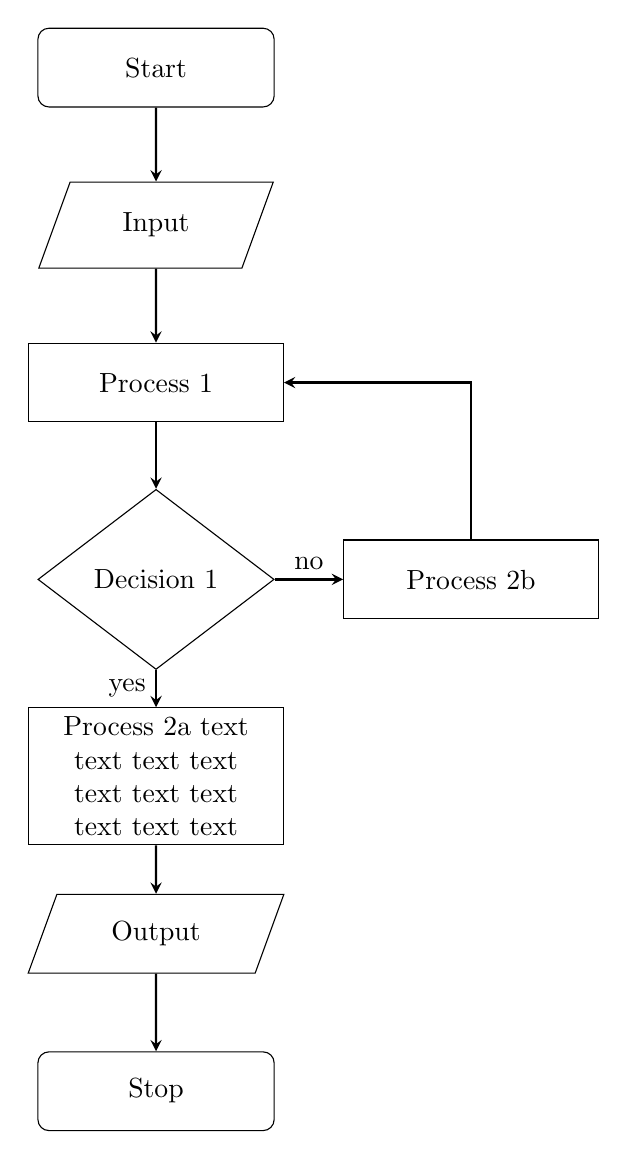
\begin{tikzpicture}[node distance=2cm]
\node (start) [startstop] {Start};
\node (in1) [io, below of=start] {Input};
\node (pro1) [process, below of=in1] {Process 1};
\node (dec1) [decision, below of=pro1, yshift=-0.5cm] {Decision 1};
\node (pro2a) [process, below of=dec1, yshift=-0.5cm] {Process 2a text text text text text text text text text text};
\node (pro2b) [process, right of=dec1, xshift=2cm] {Process 2b};
\node (out1) [io, below of=pro2a] {Output};
\node (stop) [startstop, below of=out1] {Stop};
\draw [arrow] (start) -- (in1);
\draw [arrow] (in1) -- (pro1);
\draw [arrow] (pro1) -- (dec1);
\draw [arrow] (dec1) -- node[anchor=east] {yes} (pro2a);
\draw [arrow] (dec1) -- node[anchor=south] {no} (pro2b);
\draw [arrow] (pro2b) |- (pro1);
\draw [arrow] (pro2a) -- (out1);
\draw [arrow] (out1) -- (stop);
\end{tikzpicture}
\caption{Caption here.}
\end{figure}


\section{Comparison}

Table \ref{bootcomp}

\begin{table}[h]
\caption{Properties of different bootstrap methods.}
\label{bootcomp}
\begin{tabular}{lllll}
\hline
\hline
Property/requirement & Bootstrap & OB & BLB & OBLB \\
\hline
Online & No & Yes & No & Yes \\ 
Distributed & No & No & Yes &  Yes \\ 
Resampling index precompute & Yes & No & Yes & No \\ 
Req.\ bounded data & Yes & No & Yes & No \\ 
Req.\ known bound & Yes & No & Yes & No \\ 
Maintains bootstrap histogram & Yes & Yes & No & Yes \\
\hline
\hline
\end{tabular}
\end{table}




\bibliography{online_blb}{}
\bibliographystyle{plain}

\end{document}
